\chapter{Text Clustering}

\newthought{A common task in text mining is finding interesting groups of similar documents.} That is, we would like to identify documents that are similar to each other.

We've already seen a simple example of hierarchical clustering on a 2-dimensional data set. But clustering text needs some adaptations. We have been working previously with Euclidean distances, which are analogous to the distances we can measure with a ruler.

But for complex objects with many dimensions, Euclidean distances simply don't work so well anymore. Instead, one would use cosine distance. Word counts from BoW are vectors, each pointing in a direction defined by text content. Cosine distance is the angle between these vectors.

\vspace{-0.2cm}
\begin{figure}[h]
  \centering
  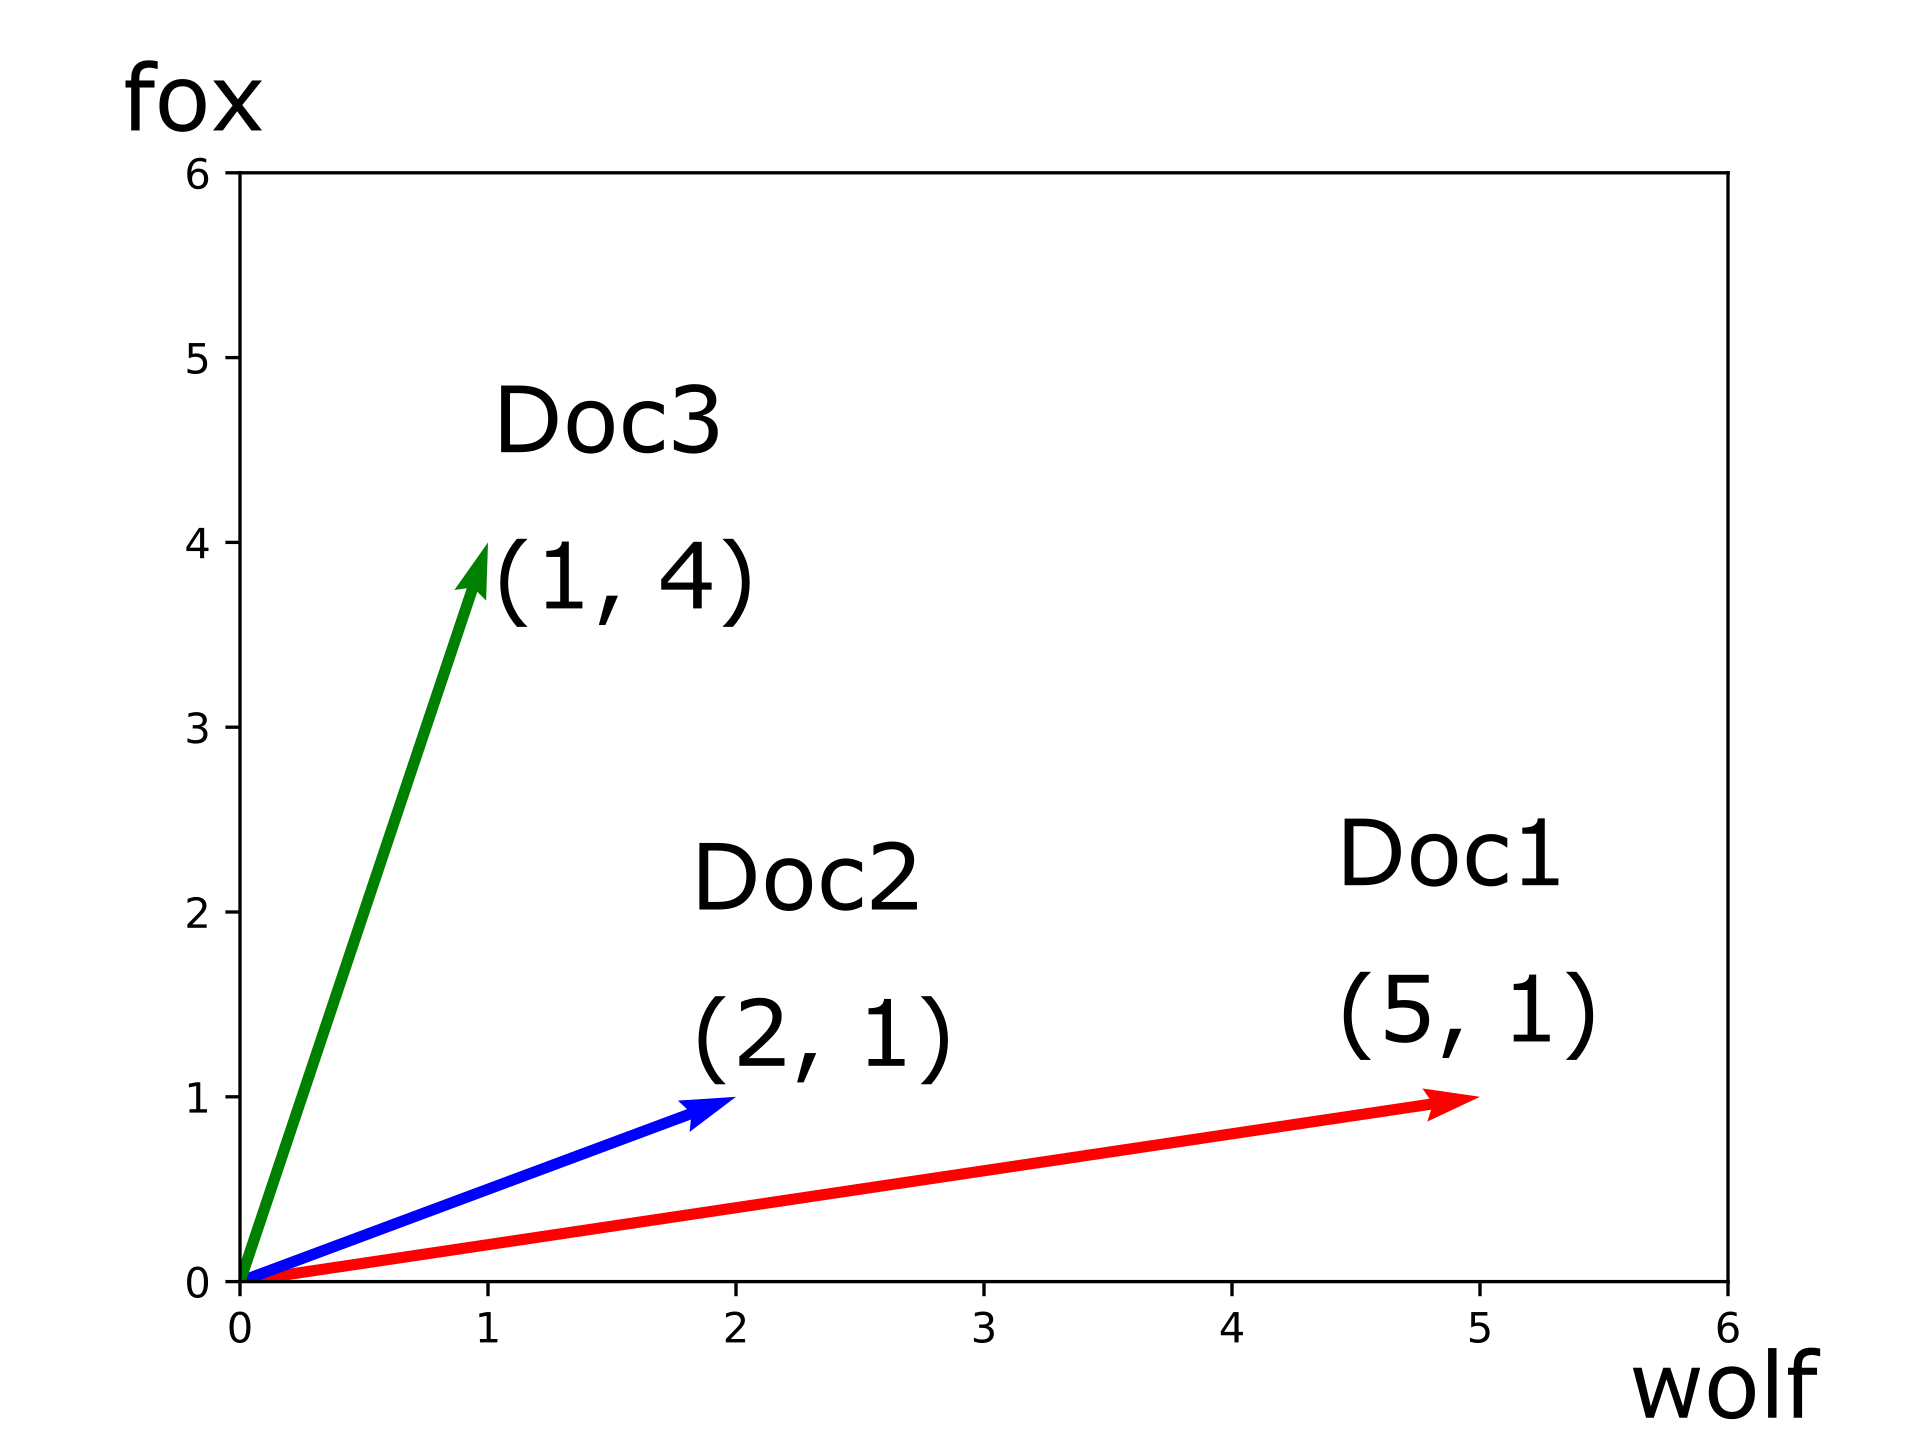
\includegraphics[width=0.9\linewidth]{cosine-distance-eng.png}%
  \caption{The plot shows vectors of three documents. Vectors correspond to the number of times the words "fox" and "wolf" appear in the text. By Euclidean distances, the two most similar documents would be Doc2 and Doc3, despite Doc2 mentioning wolves more frequently than foxes. If we take the angle between these vectors instead, Doc2 is the most similar (closest) to Doc1, which makes sense since they both talk predominantly about wolves. This is why we use the cosine distance.}
\end{figure}
\vspace{-0.3cm}

Now, let us go back to our Grimm's Tales and construct the following workflow:

\vspace{-0.2cm}
\begin{figure*}[h]
  \centering
  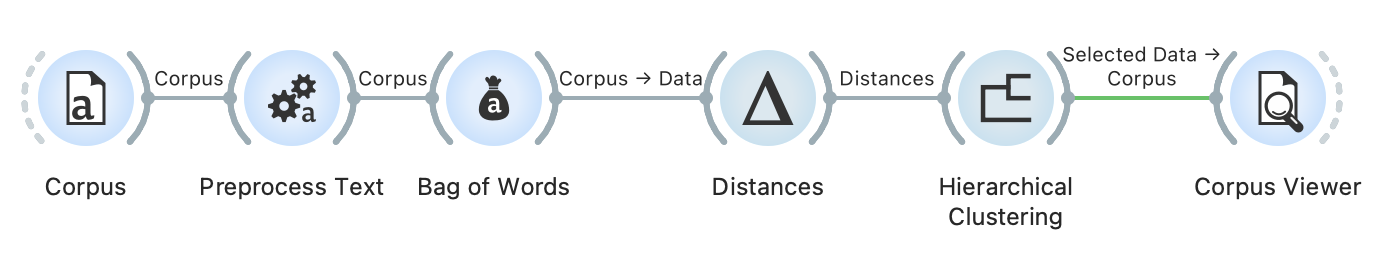
\includegraphics[width=0.9\linewidth]{workflow.png}%
  \caption{}
\end{figure*}
\vspace{-0.3cm}

\marginnote{You can try the same workflow on a different corpus, say bookexcerpt.tab, which contains excerpts from adult and children's books. }The \widget{Hierarchical Clustering widget} visualizes the clustering in a dendrogram. Connect \widget{Corpus Viewer} to Hierarchical Clustering and open both widgets. Now click on a cluster in the dendrogram and observe the documents from the selected cluster in Corpus Viewer.

Explore different clusters. Why are some Tales of Magic mixed with Animal Tales? What do they have in common?

\begin{figure*}[h]
    \centering
    \infinitewidthbox{
      \stackinset{r}{-0.35\linewidth}{t}{+0.2\linewidth}
      {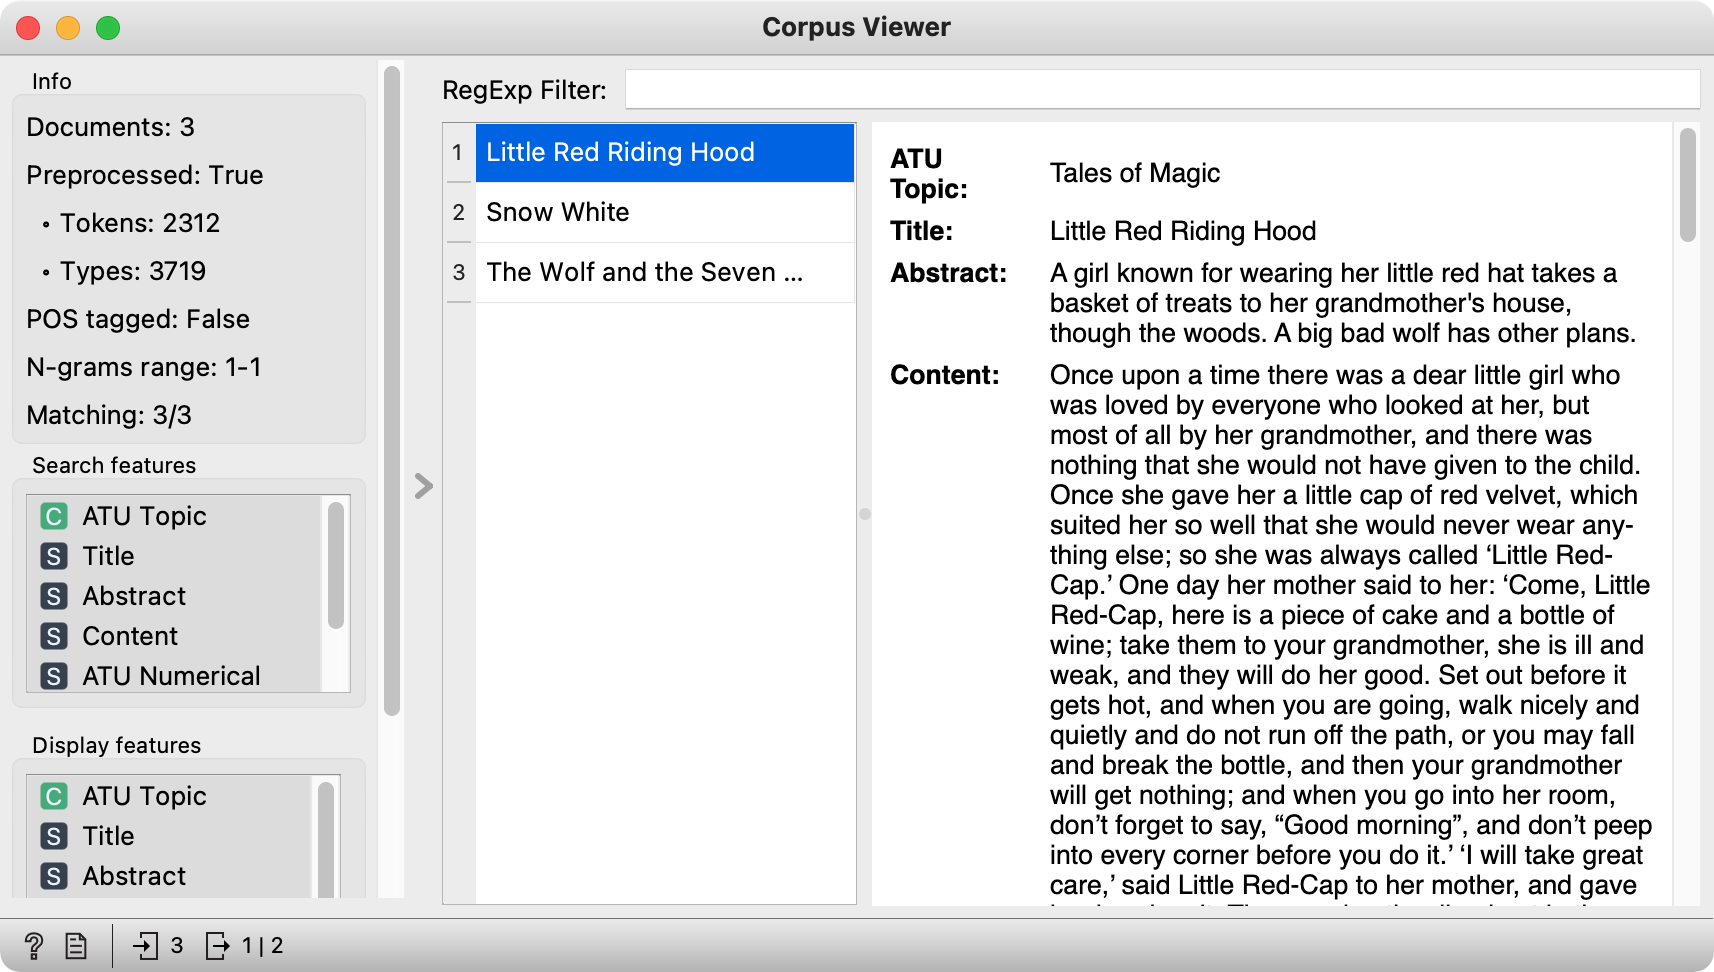
\includegraphics[scale=0.4]{corpus-viewer.png}}
      {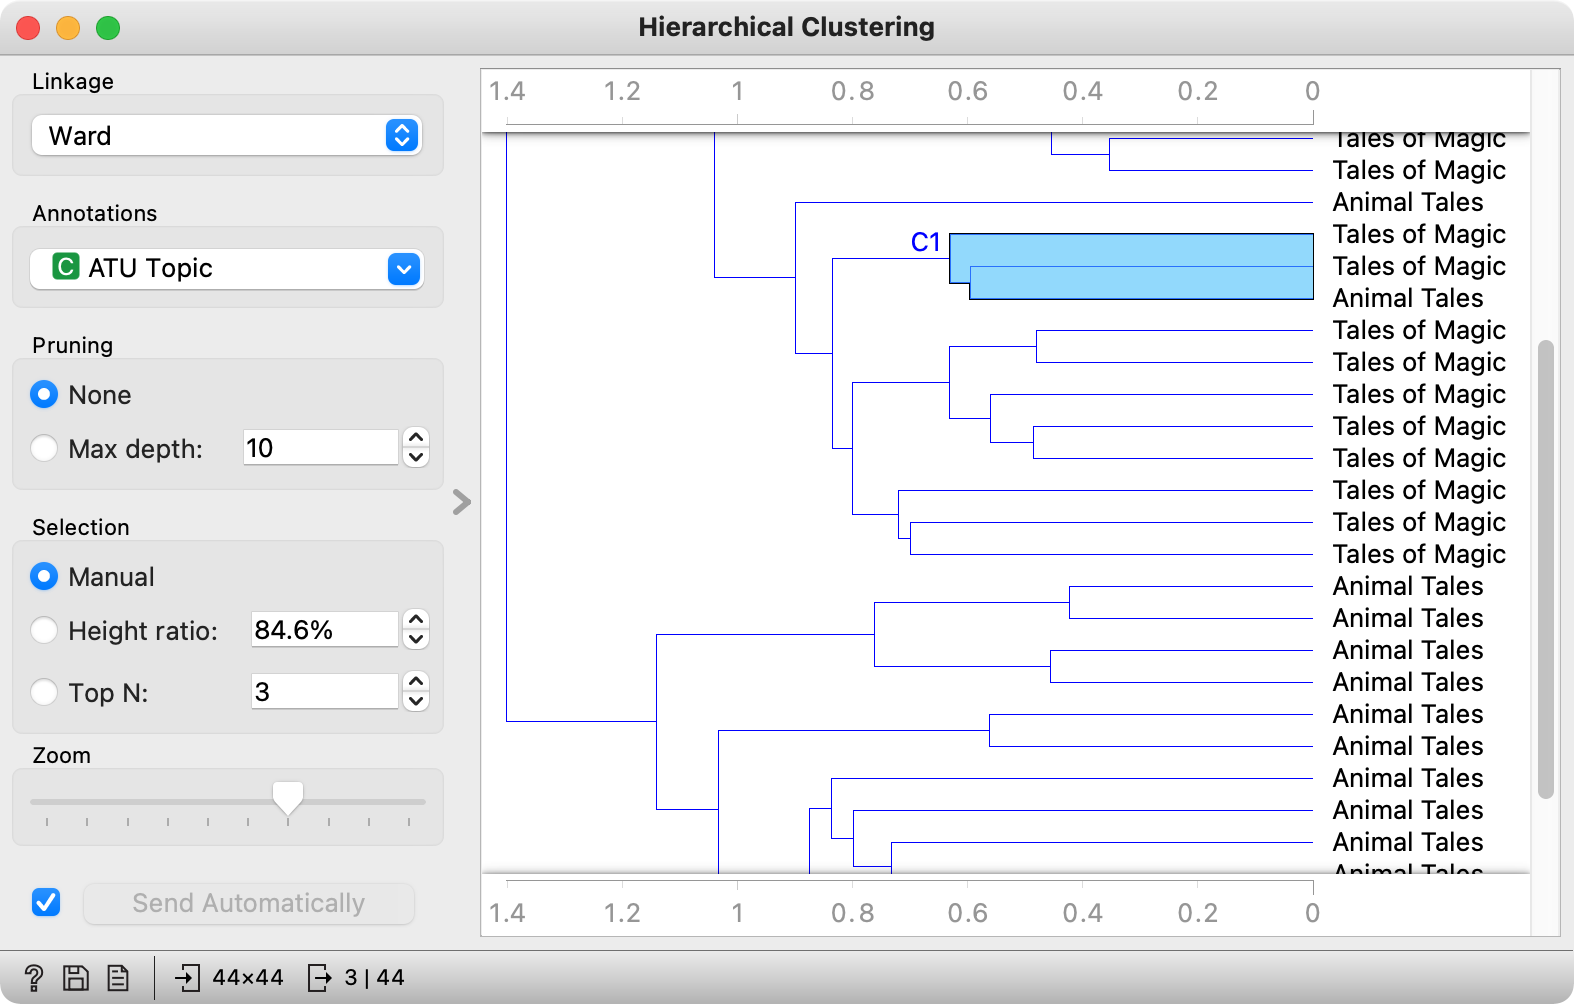
\includegraphics[scale=0.4]{hier-clust-selection.png}}
      \hspace{6cm}
      }
    \caption{$\;$}
\end{figure*}

Hierarchical Clustering builds a hierarchy of documents and it is up to us to define what is similar enough to be in one cluster. We can set the appropriate degree of similarity by dragging the vertical line left or right in the visualization.

\begin{wrapfigure}{o}{0.95\textwidth}
    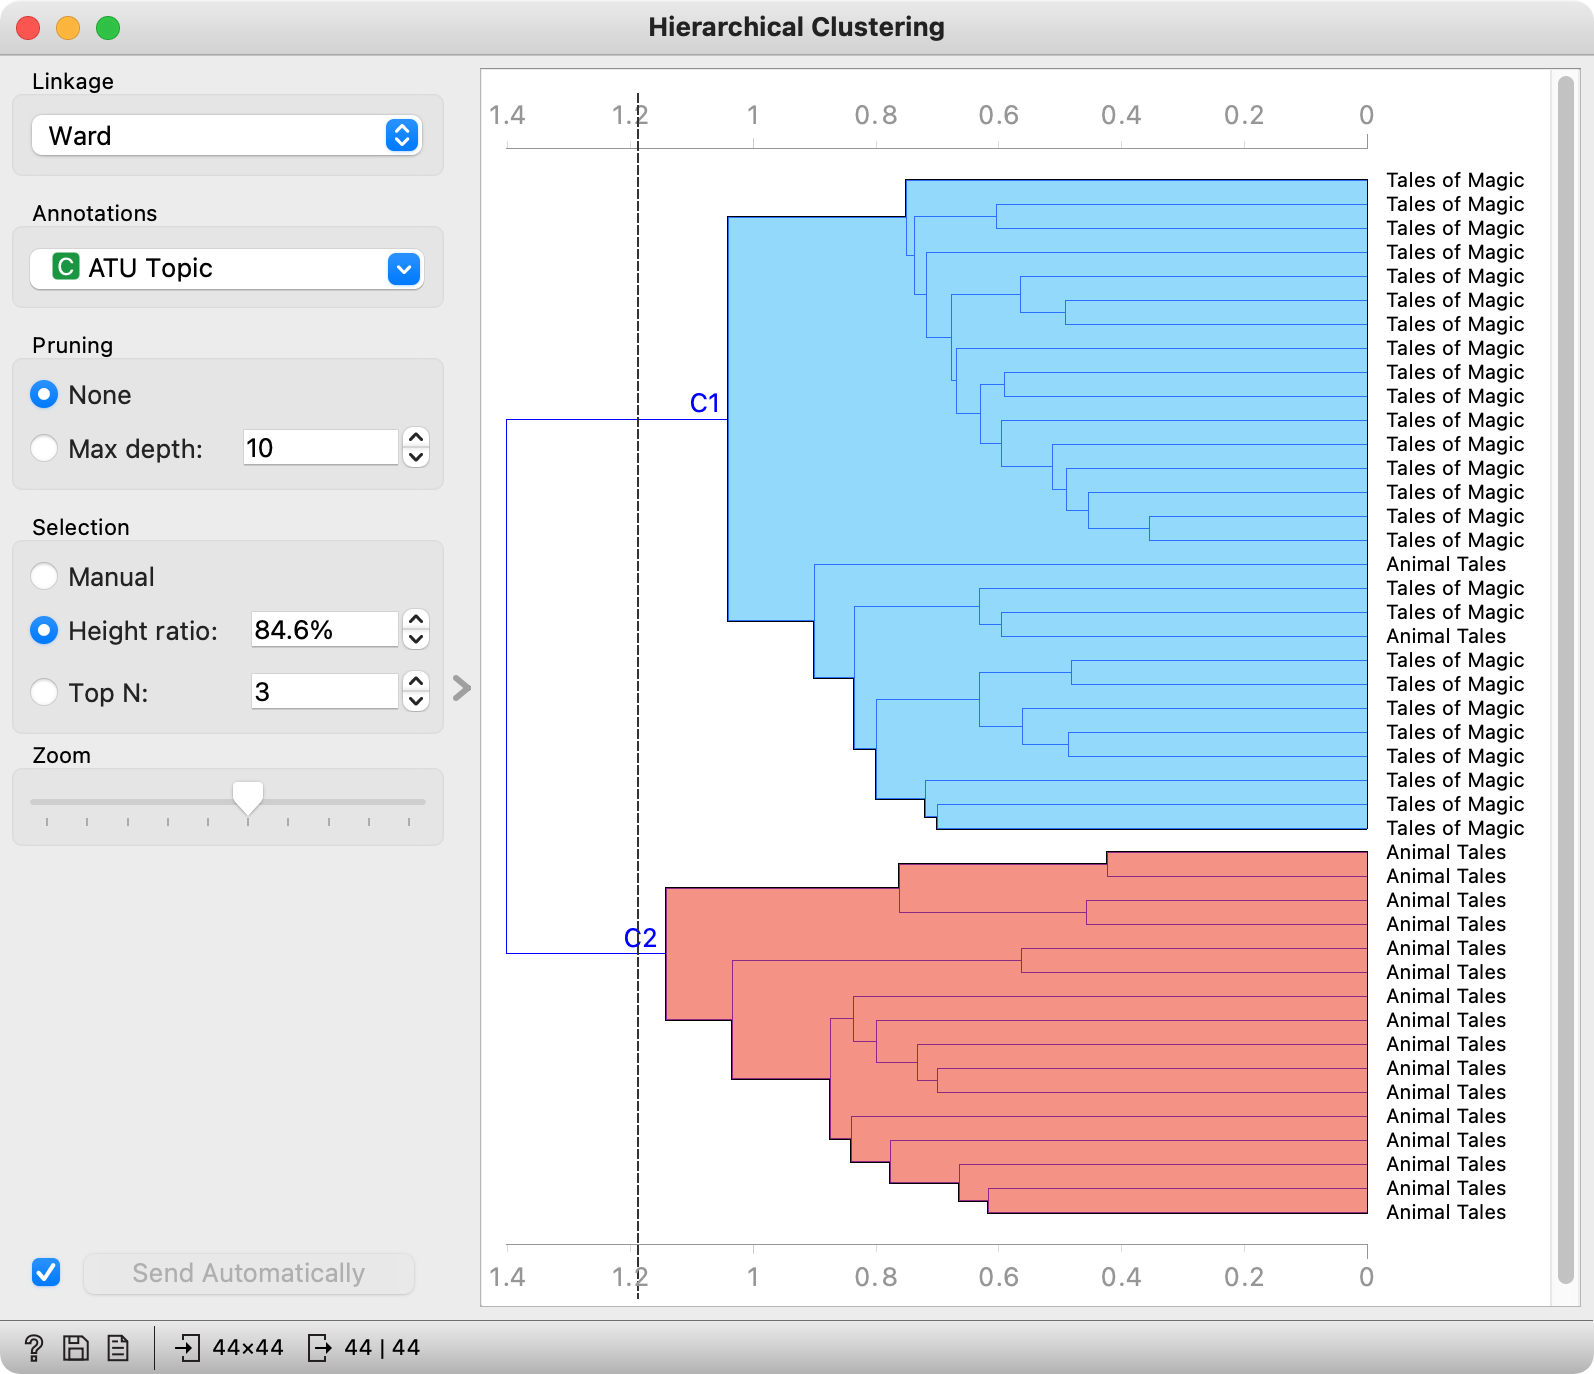
\includegraphics[scale=0.35]{hier-clust-clusters.png}
    \caption{$\;$}
\end{wrapfigure}

We went with two groups, since the distance between the clusters increases at that particular cut-off. Compare this to the cut-off we would require for three, four or five clusters. The clusters we get also correspond nicely with the designated Aarne-Thompson type (ATU Topic).

\newpage
\clearpage

But how close are the animal tales from the third and animal tales from the last cluster? Let us see the documents on a plane, where similar documents would lie close to each other. This visualization is called Multidimensional Scaling or \widget{MDS} in short.

\vspace{-0.2cm}
\begin{figure}[h]
  \centering
  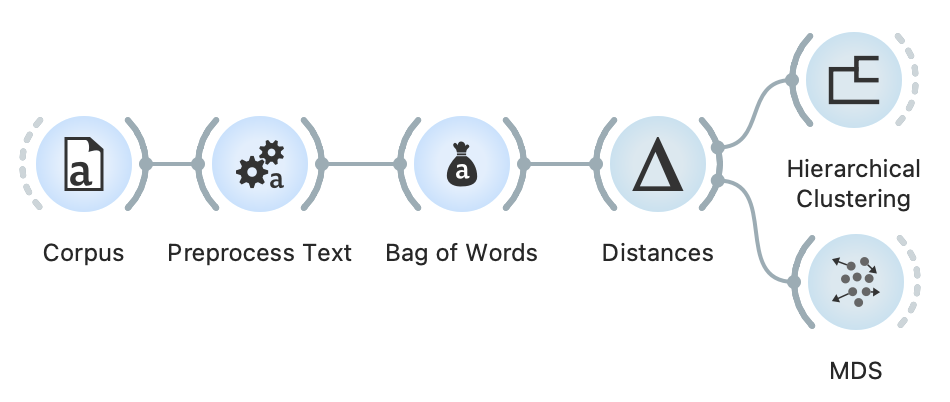
\includegraphics[width=\linewidth]{workflow2.png}%
  \caption{}
\end{figure}
\vspace{-0.3cm}

Tales of Magic form one group and Animal Tales another - just as we expected. Interestingly, Tales of Magic seem to be more similar to each other than Animal Tales are (they are connected). Inspect similar tales by selecting them in the visualization and reading them in Corpus Viewer.

\vspace{-0.2cm}
\begin{figure*}[h]
  \centering
  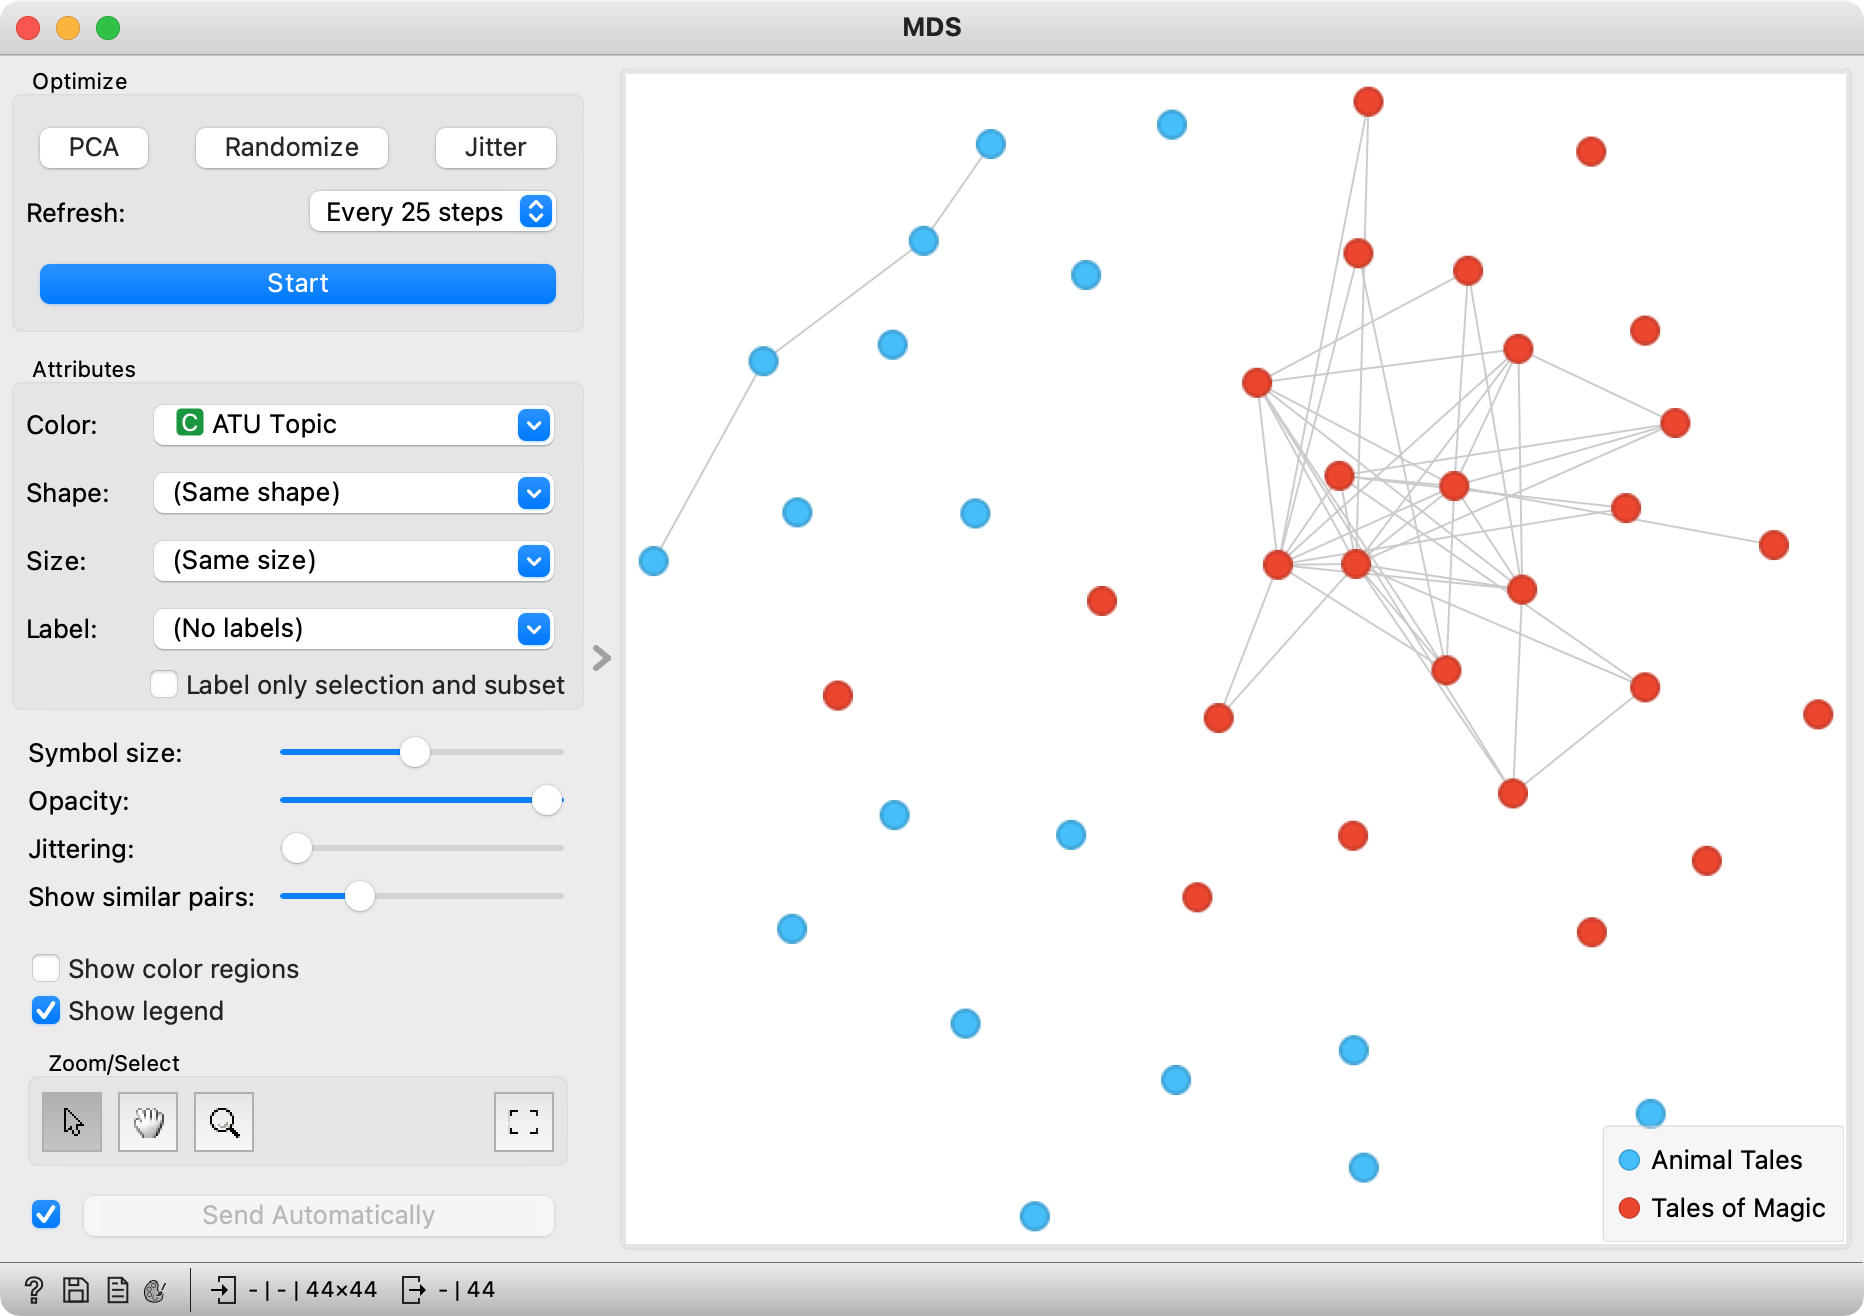
\includegraphics[width=0.9\linewidth]{mds.png}%
  \caption{}
\end{figure*}
\vspace{-0.3cm}
